Der grundsätzliche Aufbau der Suche war im Vorfeld durch das Vorhandensein im Altsystem bereits bekannt und musste nicht komplett neu konzipiert werden. Zu Beginn wurde der Code des Alt-Tools analysiert und begonnen, diesen im Admin-Relaunch in Typescript (mit React) und PHP neu zu schreiben. Beispielsweise wurden Algorithmen effizienter gestaltet und Suchkriterien optimiert. Des Weiteren wurden im Zuge des Neubaus auch Bugs gefixt.

\subsection{Model View Controller Design Pattern}
    Wie bereits in \hyperref[sec:arch]{Absatz 4.1.1} erwähnt, basieren auch die Anwendungen im Admin-Relaunch auf dem Model View Controller Design Pattern. Allerdings werden in Laravel bestimmte Bezeichnungen anders genutzt als im Altsystem.

    \subsubsection{Model, Repositories \& Libraries}
        Anders als im auf Perl und dem Framework Catalyst basierenden Altsystem, wo Models Funktionen für die Programmlogik beinhalten, sind diese im PHP-Framework Laravel vielmehr Datenbankobjekte. Diese werden mittels Eloquent, einer ORM\footnote{Object-Relational Mapping - Objektrelationale Abbildung}-Schnittstelle von Laravel, oder über den Laravel Query Builder verwendet. Jedes Model bildet eine Tabelle der Datenbank mit  all ihren Attributen ab und stellt entsprechende Zugriffsmethoden bereit. Die Eloquent- bzw. \mbox{Query} Builder-Aufrufe werden in sogenannten Repository-Klassen definiert, welche ausschließlich Funktionen für Datenbankabfragen beinhalten (näheres in \hyperref[sec:eloquery]{Absatz 5.1.4}).\\
        Diese Funktionen werden wiederum aus Library-Klassen aufgerufen, die die restliche Programmlogik beinhalten - zum Beispiel die Umformatierung von Datenstrukturen und Vorbereitung dieser zur Weitergabe an das Frontend. Somit erfüllen Libraries und Repositories noch am ehesten die Funktionen, die Models im Altsystem erfüllten.

    \subsubsection{View}
        Die View beschreibt die Ansicht der Anwendung, also das, was der Benutzer im Browser angezeigt bekommt. Die Anzeige wurde durch den Einsatz von serverseitigem Rendern via Node.js und dynamischer Anpassungen zur Laufzeit mittels React realisiert. Dabei werden per Node.js aus Typescript-Quelldateien Standard-Ansichten kompiliert und diese dann an den Client ausgeliefert. Der Gebrauch dieser Technologien hat den entscheidenden Vorteil, dass wenn sich eine Ansicht ändert, beispielsweise wenn eine Suche gestartet oder eine Unterseite aufgerufen wird, nicht die komplette Anwendung neu gerendert werden muss, sondern nur der betreffende Teil der View. Daraus ergeben sich ein geringerer Datenverkehr und insgesamt schnellere Ladezeiten.\\
        So wurde die Suchmaske in eine sogenannte \glqq Component\grqq{} ausgelagert, was bewirkt, dass diese nur beim Seitenaufruf gerendert und nicht bei jedem Event, welches auf der Seite ausgewertet wird (z. B. Nutzereingaben).

    \subsubsection{Controller}
        Der Controller nimmt, wie auch im Altsystem, nur eine vermittelnde Rolle zwischen der View und zumeist den in Library-Klassen befindlichen Funktionen ein. Controller-Funktionen werden über verschiedene API-Routen, die in der Datei \glqq api.php \grqq{} definiert sind, angesprochen. In dieser Datei wird auch die Art der Anfrage pro Route festgelegt, also ob es sich beispielsweise um eine Post- oder Get-Anfrage handelt, und werden durch das Framework auch abgewiesen, wenn die Art nicht zu der Route passt.\\
        Es wurde versucht, den Controller so schlank wie möglich zu halten und jegliche Logik in die Model-Komponenten auszulagern. Dies war ein teils stetiger Prozess, da anfangs die komplette Logik im Controller verblieb und mit wachsendem Kenntnisstand des Auszubilden ein schrittweiser Umbau vonstatten ging.

        \vspace{0.5cm}
        \begin{figure}[h]
            \centering
            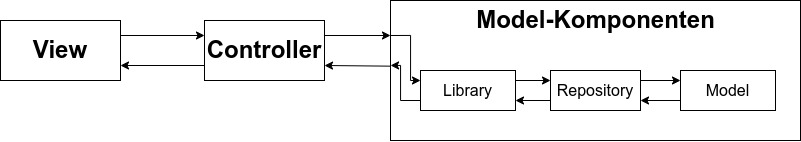
\includegraphics[width=1\textwidth]{laravel_mvc.jpg}
            \caption{MVC im PHP-Framework Laravel}
        \end{figure}

    \subsubsection{Eloquent und Query Builder}
    \label{sec:eloquery}
        Laravel stellt verschiedene Möglichkeiten bereit, Datenbankabfragen zu stellen. \glqq Eloquent\grqq{} verfolgt den objektrelationalen Ansatz. Hier werden ganze Tabellen in Objekten instanziert. Relationen und Kardinalitäten werden durch Objektmethoden dargestellt, die fest definierte Namen haben, beispielsweise \glqq hasOne()\grqq{} oder \glqq hasMany()\grqq{}. Jedoch ist Eloquent nicht so performant wie Query Builder, da es einfache Queries auf mehrere Einzelne aufteilt, sofern weitere Tabellen gejoint werden. In diesem Fall wird für jede verbundene Tabelle ein weiteres Statement ausgeführt und erst, wenn alle zugehörigen Datensätze vorliegen eine Selektion der eigentlich abgefragten Daten durchgeführt.\\
        Queries, die mit Query Builder geschrieben sind, ähneln in ihrer Syntax hingegen herkömmlichen MySQL Queries. Diese werden über eine Datenbank-Fassade verarbeitet. Die verfügbaren Funktionen sind in ihrer Benennung den SQL Keywords angelehnt. So gibt es Funktionen wie \glqq select()\grqq{}, \glqq where()\grqq{} und \glqq orderBy()\grqq{}.\\
        Aus diesem Grund ist Query Builder gerade bei großen und spezialisierten Abfragen über mehrere Tabellen weitaus leistungsfähiger, da sich der Overhead an Datenbankabfragen und übermittelten Daten auf ein Minimum reduzieren lässt.\\
        Da Eloquent-Modelle mit Query Builder kompatibel sind, kann man durchaus eine Mischform beider Ansätze verwenden.


\pagebreak

\subsection{Aufgetretene Probleme}
    Während der Projektdurchführung stieß der Auszubildende auf einen Anwendungsfall, bei dem er zuerst den Ansatz verfolgte, Datenbankabfragen per Eloquent durchzuführen, jedoch durch API-Tests und Analysen feststellte, dass eine Lösung per Query Builder weitaus performanter war. In besagtem Fall wies das Model Relationen zu weiteren Tabellen auf, aus denen je nur ein Attribut benötigt wurde. Eloquent führte jedoch 3 SQL Queries aus: eines auf die Haupttabelle und zwei weitere je auf die verbundenen Tabellen. Aus jeder Tabelle wurden komplette Datensätze abgeholt und in einem weiteren Schritt dann die eigentlich angeforderten Daten selektiert.\\
    Nach dem Umbau auf Query Builder reduzierten sich die Abfragen auf eine einzige und es wurden direkt nur die tatsächlich benötigten Daten abgeholt. Dadurch wurde die benötigte Zeit pro Abfrage um ca. 60\% reduziert.
    \vspace{0.5cm}\\
    Ein weiteres Problem stellte das dynamische Befüllen des Selects für die Abteilungsauswahl dar. Die verschiedenen Abteilungen im Unternehmen sind hierarchisch organisiert. Zum Beispiel ist der Abteilung \glqq Finance/HR/Legal\grqq{} die Abteilung \glqq Campus\grqq{} und dieser wiederum die Abteilung \glqq IT Education\grqq{} untergeordnet. Diese Hierarchie sollte ebenfalls in der Auswahl und auch in den Suchergebnissen dargestellt werden. Um dies zu realisieren, wurden die Datensätze der Abteilungen zuerst aus der Datenbank ausgelesen und danach durch eine sich rekursiv aufrufende PHP-Funktion in ein multidimensionales Objekt geschrieben. Anschließend wurde dieses an das Frontend ausgeliefert, wo es wieder durch eine rekursiv aufgerufene Funktion ausgelesen wurde. Mit jeder Ebene, die im Objekt tiefer abgestiegen wurde, wurde dem im Select angezeigten String ein \glqq $>$\grqq{} vorangestellt, um so die Hierarchieebene optisch darzustellen.%Hier Screenshot einfuegen
    \vspace{0.5cm}\\
    Eine weitere Schwierigkeit war das Abrufen der Profilbilder. Da diese nicht direkt im Frontend durch simple Angabe des Quellpfades eingebunden werden können, weil dieses keine Zugriffsberechtigung auf das entsprechende Verzeichnis hat, musste ein anderer Weg gefunden werden. So wurde zuerst versucht, über eine eigene API-Anfrage einen Binary Blob der Bilder an das Frontend zu schicken, was prinzipiell auch funktioniert hat. Jedoch konnten die React-Elemente zum Anzeigen von Bildern damit nicht umgehen. Also wurden die Bilder erst base64-codiert und anschließend im Frontend in Image-Elemente eingebunden, was zum gewünschten Ergebnis führte. Abschließend wurde der erzeugte String des Bildes noch direkt an den zugehörigen Datensatz mit den Mitarbeiterdaten angefügt und so die Requests, welche das Frontend an das Backend stellt, erheblich reduziert.
    \vspace{0.5cm}\\
    Eine Anforderung der Fachabteilung war, dass das deutsche Datumsformat verwendet wird, obgleich das restliche Tool englisch gehalten wird. Nach der anfänglichen Verwendung einer eigens geschriebenen Funktion, welche das Datum vom in der Datenbank vorliegenden amerikanischen auf das deutsche Format ändert, hat der Auszubildende sich dazu entschieden, die bereits existierende Funktion \glqq parse()\grqq{} aus der PHP Klasse \glqq Carbon\grqq{} zu verwenden. Zum einen wird dadurch redundanter Code vermieden, zum anderen ist man damit beim Format des Eingabewertes flexibler.
